\section{\scshape M. nieparametryczne}

\begin{frame}{Wady i zalety metod parametrycznych}
	\note{W idealnym dla naukowca świecie badane przez niego wartości podlegają dokładnie jednemu z typowych rozkładów matematycznych, który jest z góry znany. Niestety w praktyce rozkład trzeba zgadywać, a dane z reguły i tak nie będą do niego idealnie pasować. Rzeczywiste rozkłady są z reguły dużo bardziej złożone, ponieważ składa się na nie wiele czynników, a rozkłady teoretyczne pozwalają uwzględnić tylko część z nich, którą uznamy za najważniejszą. Takie przybliżenie może być wystarczająco dokładne, ale nie musi. Z drugiej strony jeżeli uda nam się dopasować rozkład, to otrzymujemy dużo lepsze rezultaty, to znaczy potrzebujemy mniejszej próby do wyciągania wniosków z taką samą pewnością}
	Wady:
	\begin{itemize}
		\item Wymagają znajomości lub zgadywania rozkładu
		\item Rzadko pasują idealnie do danych
		\item Mała odporność na odstające wartości
	\end{itemize}
	Zalety:
	\begin{itemize}
		\item Posiadają większą moc testów
		\item Przy dobrym doborze rozkładu wyniki mają wysoką istotność
	\end{itemize}
\end{frame}

\begin{frame}{Metody nieparametryczne - dlaczego?}
	\note{Skala interwałowa - skala, w której różnica liczbowa między dowolnymi dwoma punktami odpowiada takiej samej praktycznej różnicy między dwoma innymi, dowolnymi punktami, między którymi występuje taka sama różnica liczbowa}
	\begin{itemize}
		\item Nie wymagają zakładania żadnego rozkładu
		\item Nie wymagają dużych prób
		\item Nie wymagają weryfikacj próby pod względem podlegania rozkładowi
		\item Nie wymagają, aby pomiar dokonywany był w skali interwałowej
	\end{itemize}
\end{frame}

\begin{frame}{Metody nieparametryczne - co to jest?}
	\note{Parametry metod nieparametrycznych dotyczą sterowania działaniem algorytmu, a nie samych danych. Ogólnie typy testów nieparametrycznych są takie same, jak testów parametrycznych.}
	Cechy:
	\begin{itemize}
		\item Niezależne od rozkładu
		\item Tym bardziej od jego parametrów (stąd nazwa)
		\item Posiadają parametry, ale elastyczne i płynne
	\end{itemize}
	Typy testów nieparametrycznych:
	\begin{itemize}
		\item Testy różnic między grupami
		\item Testy różnic między zmiennymi
		\item Testy zależności między zmiennymi
	\end{itemize}
\end{frame}

\begin{frame}{Ogólna zasada działania metod nieparametrycznych}
	\note{1. Prawdopodobieństwo, że losowy punkt x znajdzie się w przedziale R
\\2. Prawdopodobieństwo, że wybierając n takich punktów, dokładnie k z nich trafi do przedziału R
\\3. Oczekiwana liczba k punktów trafiających do przedziału R
\\Przy takim rozkładzie k wartości bliskie wartości oczekiwanej są bardzo prawdopodobne, więc przybliżenie k wartością oczekiwaną k jest dość dokładne. Pozwala to wyznaczyć z dużą pewnością prawdopodobieństwo trafienia w przedział jako $k/n$. }
	\begin{equation}
		P = \int\limits_{R}p(x')dx'
	\end{equation}
	\\więc
	\begin{equation}
		P_k = {n \choose k}P^{k}(1-P)^{n-k}
	\end{equation}
	\\więc
	\begin{equation}
		\varepsilon[k] = nP
	\end{equation}
\end{frame}

\begin{frame}{Ogólna zasada działania metod nieparametrycznych - c.d.}
	\note{A skoro tak, to prawdopodobieństwo w punkcie można przybliżyć jako $frac{k/n}{V}$}
	A więc w przybliżeniu
	\begin{equation}
		 \int\limits_{R}p(x')dx' \simeq p(x)V
	\end{equation}
	wtedy
	\begin{equation}
		p(x) \simeq \frac{k/n}{V}
	\end{equation}
\end{frame}

\begin{frame}{Problemy natury technicznej i teoretycznej}
	\note{$V$ musi zmierzać do 0, żeby było to dokładne prawdopodobieństwo w punkcie; $k$ musi zmierzać do nieskończoności, żeby było to dokładnie $k$ wynikające z prawdopodobieństwa; $k/n$ musi zmierzać do 0, żeby cały ułamek w ogóle mógł mieć granicę właściwą}
	\begin{itemize}
		\item Przy $n\rightarrow\infty$ i stałym $V$ jest to uśrednione lokalnie prawdopodobieństwo
		\item Przy $V\rightarrow0$ i stałym $n$ przedziały przestają obejmować jakiekolwiek próby
		\item Nawet teoretycznie mając $V\rightarrow0$ i $n\rightarrow\infty$ spełnione muszą być warunki:
		\begin{itemize}
			\item \[\lim_{n\to\infty}V_n = 0 \]
			\item \[\lim_{n\to\infty}k_n = \infty \]
			\item \[\lim_{n\to\infty}k_n/n = 0 \]
		\end{itemize}
	\end{itemize}
\end{frame}

\begin{frame}{(Względnie najprostszy) przykład - histogram}
	\note{Do jednego z najprostszych przybliżeń rozkładu można posłużyć się histogramem. Tutaj dane jest 20 losowych wartości, które dzielimy między przedziały o szerokości 10.}
	$n = 20$
	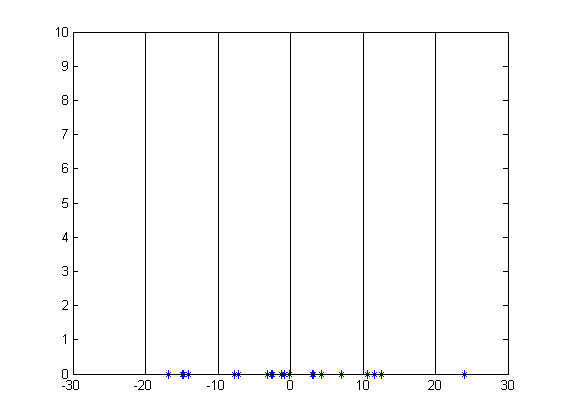
\includegraphics[keepaspectratio=true,scale=0.6]{pre}
\end{frame}

\begin{frame}{Przykład c.d.}
	\note{Do kolejnych przedziałów histogramu trafia odpowiednio 0, 4, 8, 4, 3 i 1 próbek. Można więc przybliżać prawdopodobieństwo, że inne zmienne losowe będą się znajdować w kolejnych przedziałach do 0.0 (0/20), 0.2 (4/20), 0.4 (8/20), 0.2 (4/20), 0.15 (3/20) i 0.05 (1/20). Nie jest to zbyt efektywna metoda, ale dobrze przedstawia ideę, która jest bardzo podobna między innymi w następnej omawianej metodzie nieparametrycznej, oknie Parzen.}
	$n = 20$
	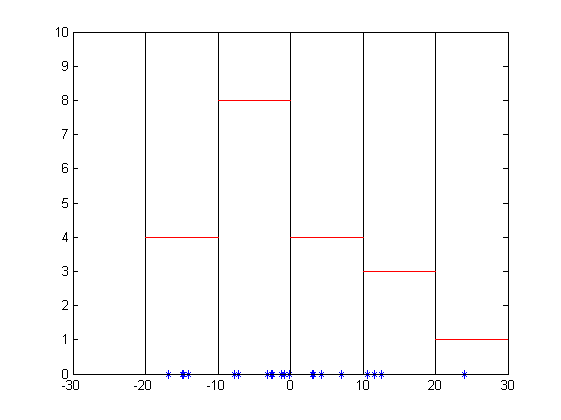
\includegraphics[keepaspectratio=true,scale=0.6]{post}
\end{frame}